
% Commonly-used LaTeX commands in this book:
%%%
%%% \chapter{Title of Chapter}
%%%   \section{Title of Section}
%%%   \section*{Title of non-numbered Section (example: Bibliographies)}
%%%   \subsection{Title of Subsection}
%%%   \subsubsection{Title of Sub-subsection}
%%%
%%% (My convention in this book is to precede each sectioning command with a 
%%% \filbreak command to prompt a new page, with the exception of chapters
%%% and subsubsections.  
%%%
%%% \index{Index entry here . . .}
%%%
%%% \footnote{Footnote text here . . .}
%%%
%%% $$\includegraphics{name_of_graphics_file.eps}$$
%%% $$\includegraphics[width=5in]{name_of_graphics_file.eps}$$
%%%
%%% \textit{Text set in ``bold'' font}
%%% \textbf{Text set in ``bold'' font}
%%% \texttt{Text set in ``typewriter'' font}
%%%
%%% \begin{itemize}
%%%   \item First item
%%%   \item Second item
%%%   \item Third item
%%%   \subitem First subitem under third item
%%%   \subitem Second subitem under third item
%%% \end{itemize}
%%%
%%% \begin{enumerate}
%%%   \item First numbered item
%%%   \item Second numbered item
%%%   \item Third numbered item
%%% \end{enumerate}
%%%
%%% \begin{quotation}
%%%   Paragraph 1
%%%   Paragraph 2
%%%   Paragraph 3
%%% \end{quotation}
%%%
%%% \begin{quote}
%%%   Paragraph (one paragraph only!)
%%% \end{quote}
%%%
%%% \newpage
%%%
%%% \label{Text name of label}   (used to identify things to reference)
%%% \ref{Text name of label}     (used to generate section cross-references)
%%% \pageref{Text name of label} (used to generate page references)
%%%
%%%\lstset{language=pseudocode}   OR   \lstset{language=C}
%%%\begin{lstlisting}[mathescape] ("mathescape" allows the use of $\symbols$ inside the code listing)
%%%   (Insert source code here)
%%%\end{lstlisting}




%%%% Things to do for future versions %%%%

% ADD: tunable laser diode (TLD) absorption spectrometer for gas analysis

% ADD: illustration of a Foxboro E69 I/P converter with motion-balance design

% ADD for future versions: circuit-sketching techniques 
  % --> \subsection{Determining proper wire connections in signal circuits}

% ADD for future versions: complete transfer function analysis in Basic Process Control Strategies chapter

% ADD: motor starting methods subsection 

% ADD: solid-state motor starter subsection 









\documentclass[12pt,a4paper,margin=2cm]{book}





% The "ulem" package enables the use of ``strike-out'': e.g. \sout{Text to be struck}
\usepackage{ulem}

% The "makeidx" package enables the creation of an index for the book
\usepackage{makeidx}

% The "graphicx" package allows image widths to be specified: e.g. \includegraphics[width=4in]{junk.eps} 
\usepackage[dvips]{graphicx} 

% The "array" package allows manipulation of table row height using the "extrarowheight" setlength option
\usepackage{array}
\usepackage{amsmath}

\usepackage{xcolor}

% The "listings" package enables programming source code to be formatted in an attractive way
\usepackage{listings}
\usepackage{makecell} % gjør det mulig å gjøre linjebytte i en enkelt celle \makecell{}
% The "hyperref" package enables hyperlinks in the dvi, PostScript, and PDF output files
% for easier navigation.  This includes hyperlinked index and TOC entries!
\usepackage[
	pdftitle = "{Automatiseringssystemer For Gand VGS}",
    pdfauthor = "{Fred-Olav Mosdal}",
%    dvips = false,
%    ps2pdf = false,
%    pdftex,
    colorlinks = true,
    breaklinks= true,
    hyperindex = true
]{hyperref}


\setlength{\parskip}{1em}
\setlength{\parindent}{0em}


% These commands set widths of text, and margins:
\setlength{\textwidth}{16cm}
\setlength{\evensidemargin}{0cm}
\setlength{\oddsidemargin}{0cm}
\setlength{\extrarowheight}{3pt} % adds extra space to the top of each LaTeX ("tabular") table row to make superscripted math expressions look better

% This command prompts the compilation of an index
\makeindex









% This begins the document:
\begin{document}


% This line effectively turns off "Underfull \vbox" and "Underfull \hbox" error messages.
\hbadness=20000
\vbadness=20000

\tolerance = 1000
\pretolerance = 10000



% Define "pseudocode" as a language recognized by the "listings" package:
\lstdefinelanguage{pseudocode}
{morekeywords={DECLARE,BEGIN,END,LOOP,ENDLOOP,SET,IF,THEN,CALL,RETURN,ELSEIF,ELSE,ENDIF,PRINT,OUTPUT,AND,OR},
 morecomment=[l]{//}
}

\lstloadlanguages{pseudocode,[ANSI]C}

% Set some of the environment variables for the "listings" package to format source code:
%\lstset{frame=single,language=pseudocode,keywordstyle=\color{blue}\bfseries,commentstyle=\color{red}\itshape}
\lstset{frame=single,keywordstyle=\color{blue}\bfseries,commentstyle=\color{red}\itshape}









%% Cover %%

\begin{titlepage}

\begin{center}

\textsc{\LARGE Automatiseringssystemer for Gand VGS }

%$$\includegraphics[width=16cm]{cover.eps}$$

\textsc{\copyright{} 2020 by Fred-Olav Mosdal-- under the terms and conditions of the Creative Commons Attribution 4.0 International Public License}

\vskip 20pt

%\textsc{Version 2.16 (stable) -- Released January 1, 2016}
\textsc{Version 0.01 (development) -- Last update April 29, 2020}

\end{center}

\end{titlepage}






%% Copyright page %%

\pagenumbering{roman}

\textsl{Lessons In Industrial Instrumentation} \copyright{} 2008-2018 by Tony R. Kuphaldt

\vskip 10pt

This book is a copyrighted work, but licensed under the Creative Commons Attribution 4.0 International Public License.  To view a copy of this license, turn to Appendix \ref{CC_license}, or visit \texttt{http://creativecommons.org/licenses/by/4.0/} or send a letter to Creative Commons, 171 Second Street, Suite 300, San Francisco, California, 94105, USA.  The terms and conditions of this license allow for free copying, distribution, and/or modification of all licensed works by the general public.

\vskip 20pt

%\textbf{Revision history}\footnote{Version numbers ending in odd digits are developmental (e.g. 0.7, 1.23, 4.5), with only the latest revision made accessible to the public.  Version numbers ending in even digits (e.g. 0.6, 1.0, 2.14) are considered ``public-release'' and will be archived.  Version numbers beginning with zero (e.g. 0.1, 0.2, etc.) represent early editions that were substantially incomplete.}
%
%\begin{itemize}
%\item Version 0.1 -- July 2008 to September 2008 (initial development)
%\item Version 0.2 -- released September 29, 2008 for Fall quarter student use (SafeCreative registration code \texttt{0810111072182})
%\item Version 0.4 -- released January 12, 2009 for Winter quarter student use (SafeCreative registration code \texttt{0901122394919})
%\item Version 0.6 -- released April 21, 2009 for public use (SafeCreative registration code \texttt{0904213106101})
%\item Version 0.8 -- released September 8, 2009 for public use (SafeCreative registration code \texttt{0909094400980})
%\item Version 1.0 -- released September 28, 2009 for public use (SafeCreative registration code \texttt{0909284601913})
%\item Version 1.2 -- released January 12, 2010 for public use (SafeCreative registration code \texttt{1001125303242})
%\item Version 1.4 -- released April 11, 2010 for public use (SafeCreative registration code \texttt{1004125976416})
%\item Version 1.6 -- released May 4, 2010 for public use (SafeCreative registration code \texttt{1005046194859})
%\item Version 1.8 -- released June 1, 2010 for public use (SafeCreative registration code \texttt{1006016477958})
%\item Version 1.10 -- released June 28, 2010 for public use (SafeCreative registration code \texttt{1006286691573})
%\item Version 1.12 -- released September 20, 2010 for public use (SafeCreative registration code \texttt{1009217397803})
%\item Version 1.14 -- released January 11, 2011 for public use (SafeCreative registration code \texttt{1101118240391})
%\item Version 1.16 -- released April 11, 2011 for public use (SafeCreative registration code \texttt{1104118950581})
%\item Version 1.18 -- released July 4, 2011 for public use (SafeCreative registration code \texttt{1107069618739})
%\item Version 1.20 -- released September 19, 2011 for public use (SafeCreative registration code \texttt{1109190093232})
%\item Version 1.22 -- released January 8, 2012 for public use (SafeCreative registration code \texttt{1201090880285})
%\item Version 1.24 -- released April 8, 2012 for public use (SafeCreative registration code \texttt{1204091446627})
%\item Version 1.26 -- released June 30, 2012 for public use 
%\item Version 1.28 -- released September 18, 2012 for public use 
%\item Version 1.30 -- released January 5, 2013 for public use 
%\item Version 1.32 -- released April 1, 2013 for public use 
%\item Version 1.34 -- released July 1, 2013 for public use 
%\item Version 1.36 -- released September 23, 2013 for public use 
%\item Version 2.00 -- released January 12, 2014 for public use 
%\item Version 2.02 -- released April 14, 2014 for public use 
%\item Version 2.04 -- released August 8, 2014 for public use 
%\item Version 2.06 -- released September 22, 2014 for public use 
%\item Version 2.08 -- released January 12, 2015 for public use 
%\item Version 2.10 -- released April 7, 2015 for public use 
%\item Version 2.12 -- released June 29, 2015 for public use 
%\item Version 2.14 -- released September 21, 2015 for public use 
%\item Version 2.16 -- released January 1, 2016 for public use 
%\item Version 2.18 -- released April 11, 2016 for public use 
%\item Version 2.20 -- released September 16, 2016 for public use 
%\item Version 2.22 -- released April 8, 2017 for public use 
%\item Version 2.24 -- released July 4, 2017 for public use 
%\item Version 2.26 -- released September 25, 2017 for public use 
%\item Version 2.28 -- released April 1, 2018 for public use 
%\item Version 2.30 -- released September 12, 2018 for public use 
%\end{itemize}
%
%
%
%
%
%
%%% Table of contents %%
%
\tableofcontents  
\cleardoublepage
\pagenumbering{arabic}








%% Preface %%

\vfil \eject


%%%%%%%%%%%%%%%%%%%%%%%%%%%%%%%%%%%%%%%%%%%%%%%%%%%%
%% Begin book chapters, sections, and subsections %%
%%%%%%%%%%%%%%%%%%%%%%%%%%%%%%%%%%%%%%%%%%%%%%%%%%%%

%\input PrefaceByTony.tex
%
%\input Calculus.tex 
\input Physics.tex
%\input Chemistry.tex
%\input ACelectricity.tex
\input IntroductionToIndustrialInstrumentation.tex
\input InstrumentationDocuments.tex
\input InstrumentConnections.tex
\input DiscreteProcessMeasurement.tex
\input DiscreteControlElements.tex
\input RelayControlSystems.tex
%\input PLC.tex
\input PLS.tex
\input AnalogElectronicInstrumentation.tex
\input PneumaticInstrumentation.tex
\input DigitalDataAcquisitionAndNetworks.tex
\input FoundationFieldbusInstrumentation.tex
\input WirelessInstrumentation.tex
\input InstrumentCalibration.tex
\input ContinuousPressureMeasurement.tex
\input ContinuousLevelMeasurement.tex
\input ContinuousTemperatureMeasurement.tex
\input ContinuousFluidFlowMeasurement.tex
\input ContinuousAnalyticalMeasurement.tex
%\input MachineVibrationMeasurement.tex
%\input ElectricPowerMeasurementAndControl.tex
\input SignalCharacterization.tex
%\input InferentialMeasurement.tex  %Dead Chapter
\input ControlValves.tex
\input VariableSpeedMotorControls.tex
\input ClosedLoopControl.tex
\input ProcessDynamicsAndPIDControllerTuning.tex
\input BasicProcessControlStrategies.tex
\input ProcessSafetyAndInstrumentation.tex
\input InstrumentationCyberSecurity.tex
\input ProblemSolvingAndDiagnosticStrategies.tex
%\input FlipBookAnimations.tex
%\input DoctorStrangeflow.tex
%\input DisassemblyOfaSlidingStemControlValve.tex
%\input HowToUseThisBook.tex
%\input Contributors.tex
\input CreativeCommonsAttributionLicense.tex



%%%%%%%%%%%%%%%%%%%%%%%%%%%%%%%%%%%%%%%%%%%%%%%%%%%%

%%%%%%%%%%%%%%%%%%%%%%
%% Begin book index %%
%%%%%%%%%%%%%%%%%%%%%%

\printindex



%% The end! %%
\end{document}
\end{book}


